\documentclass{article}
\title{Assignment: A Non-parametric Bayesian Model for Word Segmentation}
\author{Sander Nugteren\\ 6042023 \and Ties van Rozendaal\\ 10077391 \and Joost Baptist\\ 10760105}
\date{\today}

\usepackage{amsmath}
\usepackage{algorithm}
\usepackage[noend]{algpseudocode}
\usepackage{bm}
\usepackage{amsfonts}
\newcommand{\vt}[1]{\bm{\mathbf{#1}}}
\newcommand{\zmin}[0]{\vt{z}_{-i}}
\newcommand{\wmin}[0]{\vt{w}_{-i}}
\makeatletter
\def\BState{\State\hskip-\ALG@thistlm}
\makeatother

\begin{document}

\maketitle

\section{Introduction}
The problem of how infants learn to identify individual words in spoken language has been the topic of many research projects for some time now. Since words in a sentence are rarely spoken in isolation (i.e. with pauses in between), there is no trivial way for infants to learn where word boundaries are. This has caused researchers to suspect that infants actually employ statistical strategies as a first step in learning word boundaries, in which statistical regularities play an important role \cite{thiessen2003cues}.

Early work on statistical word segmentation relies on the observation that transitions between syllables or phonemes are generally less predictable at word boundaries than within words (\cite{harris1970phoneme}, \cite{saffran1996statistical}), which can give the learner a cue as to whether or not there should be word boundary. Behavioural research has shown that infants are sensitive to this effect \cite{saffran1996statistical} \cite{aslin1998computation}. This gives rise to the assumption that words are units that, to some degree, help predict other units in a sentence.

\cite{Goldwater200921} proposed a Bayesian framework for the statistical word segmentation problem with the goal to identify the assumptions the learner must make in order to correctly segment (real) natural language. They investigate what kind of words learners with different assumptions are able to identify, using a corpus of phonetically transcribed child-directed speech. Specifically, they test the hypothesis that words are statistically independent units, to which end they developed two different models.

The first model is a unigram model: it treats each word independently (i.e. words do not predict later words). They find that this model has a tendency to undersegment the corpus, by identifying frequently co-occuring sequences as a single word. For example, because sequences like \textit{would you} and \textit{that's a} are relatively common, the learner may be tempted to classify these sequences as single words (i.e. \textit{wouldyou} and \textit{thatsa}).

The second model is a bigram model that assumes that words can predict later words. That is, this model assumes that the choice of a word is conditioned on the previous word. Because of this assumption this model is able to greatly reduce the problem of undersegmentation.

Both models in \cite{Goldwater200921} use a (hierarchical) Dirichlet Process (DP) to define probabilities over clustering of word tokens. The Dirichlet process integrates over the number of clusters $K$, and therefore is useful when $K$ is unknown. The probability of assigning a new datapoint $z_i$ to an existing cluster $k$, is proportional to the size of that cluster. The exact probabilities are given by:
\begin{align}
P(z_i=k|\zmin) = 
\begin{cases}
    \frac{n_k^{(\zmin)}}{i - 1 - \alpha},& 1 \le k \le K(\zmin)\\
    \frac{\alpha}{i - 1 - \alpha}              & k = K(\zmin)\\
\end{cases} \label{eq:DP}
\end{align}
where $\zmin$ are the clusters without datapoint $i$, and $n_K^{(\zmin)}$ is the number datapoints assigned to the cluster $k$.

Even though the DP has been found very useful in clustering, the distributions that it prefers do not match the powerlaw distributions that are usually observed over types and tokens. In order to make the DP more suitable for these word distributions, the Pitmann-Yor process (PYP) \cite{pitman1997two} introduces a discount factor $\beta$. The probabilities for clustering become:
\begin{align}
P(z_i=k|\zmin) = 
\begin{cases}
    \frac{n_k^{(\zmin)} - \beta}{i - 1 - \alpha},& 1 \le k \le K(\zmin)\\
    \frac{\alpha + \beta K}{i - 1 - \alpha}              & k = K(\zmin)\\
\end{cases}  \label{eq:PYP}
\end{align}
Indeed, the distributions generated by the PYP model are very close to the empirical distributions of types and tokens \cite{goldwater2005interpolating}.

\todo[inline]{nog meer over model omschrijven?}

The goal of this project is to reproduce the unigram model by \cite{Goldwater200921} and to replicate their results. We experiment with different intialization strategies and parameter values and show their effect on precision, recall and the $F_0$-measure. In a qualitative analysis we show that the unigram model does indeed have a tendency to undersegment the corpus. Finally, we discuss the merits and shortcomings of this model. 

We also implement a unigram model based on the PYP process. We compare this model to the DP unigram model, and investigate the effect of different parameters using a grid search. The DP model structurally outperforms the PYP model. We discuss why this happens, and suggest improvements for this model.

\section{Model}

\section{Experiments}

\subsection{Evaluation metrics}

Following \cite{Goldwater200921}, we define two types of evaluation metrics: the joint probability of the corpus and retrieval measures.

\subsubsection{Corpus probability}

For the DP model, the joint probability over all the words in the corpus is defined for as follows:

\begin{equation}
p(\mathbf{w} | \alpha, P_0) = \prod_{w_i \in \mathbf{V}} \left( \frac{n_{w_i} - 1 + \alpha P_0(w_i)}{N - 1 + \alpha} \right)^{n_{w_i}}
\end{equation}

where $\mathbf{V}$ is the lexicon or vocabulary, $N$ is the total number of words in the corpus, and $n_{w_i}$ is the number of occurences of word $w_i$ in the corpus.

\subsubsection{Retrieval measures}

We assess the quality of the retrieved segmentation using precision, recall and the $F_0$ measure. Like \cite{Goldwater200921}, we evaluate these measures on words (per utterance), on boundaries (per utterance, excluding the start and end of the utterance), and on the lexicon. This gives us nine retrieval measures for each experiment.

\subsection{$P_0$ distribution}

$P_0$ is the prior distribution over phonemes. We experiment with a uniform distribution ('uniform'), and one that is based on proportional counts in the corpus ('mle'). We evaluate using the log joint probability over time.

\subsection{Gibbs sampling}

The retrieved segmentation depends in part on the Gibbs sampling procedure. We experiment with different temperature regimes and initialisation strategies. Like the choice of $P_0$ distribution, we evaluate the temperature regimes and initialisation strategries using the log joint probabiliy over time.

\subsubsection{Temperature regime}

We experimented with three different temperature regimes:

\begin{itemize}
\item Regime 0: 20000 iterations, from 0.1 to 1 in evenly spaced steps of 0.1
\item Regime 1: 30000 iterations, from 0.1 to 1.5 in evenly spaced steps of 0.1
\item Regime 2: 40000 iterations, from 0.002 to 1 in evenly spaced steps of 0.002
\end{itemize}

\subsubsection{Initialisation}

In all experiments, the boundaries are initialised randomly. We experimented with the proportion of boundaries that were initialised with respect to the total number of possible boundaries (per utterance). We tested proportions $0$, $\frac{1}{3}$, $\frac{2}{3}$, $1$.

\subsection{Model parameters}

The parameters of the DP model are $\alpha_0$, which affects the number of word types proposed, and $p_\#$, the prior probability of a word boundary. We experiment with $\alpha_0 \in \{1, 2, 5, 10, 20, 50, 100, 200, 500\}$ and $p_\# \in \{0.1, 0.3, 0.5, 0.7, 0.9\}$. During the $\alpha_0$ experiments we kept $p_\#$ fixed to 0.5 and during the $p_\#$ experiments we kept $\alpha_0$ fixed to 20.

\subsection{PYP Model}

Because $h^{-}$ has to be modelled explicitly in the PYP model, the sampling is computationally a lot more expensive than the sampler used in DP sampling. Therefore a different iteration scheme was used with only 4000 iterations, and three equal temperature steps (0.1, 1.1, 1.6).

\subsubsection{Algorithm}
Because the Gibbs sampling in the PYP model is slightly more complicated than the sampler for the DP model, some experiments were run, to test wether the sampler was implemented correctly.
First, the PYP model was run with the $\beta$ parameter set to 0. The results were compared to the DP model with the exact same parameters and temperature regime. Both models were expected to produce the same results.

Next, the probability of the corpus was calculated and examined after each iteration. If the sampler was implemented

\subsubsection{Parameters}
Both the concentration paramter $\alpha$ and the smoothing paramter $\beta$ effect the seating distribution and might therefore interact with eachother. In order to find the best settings for $\alpha$ and $\beta$, a grid search was conducted with $\alpha \in \{1, 2, 5, 10, 20, 50, 100, 500 \}$ and $\beta \in \{ 0.01, 0.1, 0.2, 0.4,0.6, 0.8, 1, 0 \}$

\section{Results}

\subsection{$P_0$ distribution choice}

Figure \ref{fig:P0_logprob} shows the effect of phoneme distribution choice on the log joint probability. It turns out that the choice hardly influences the log joint probability at all.

\begingroup
    \centering
    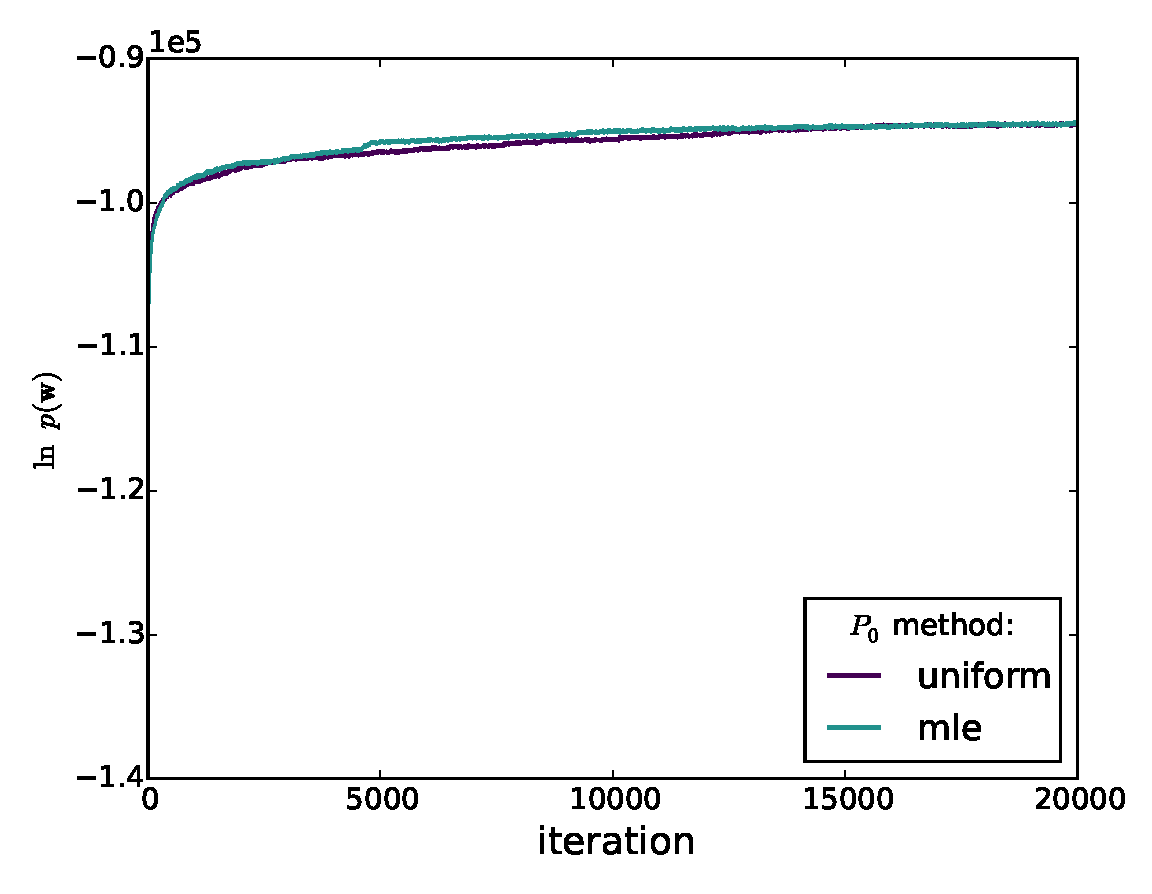
\includegraphics[width=0.5\textwidth]{images/P0_method-log_prob}
    \captionof{figure}{The effect of phoneme distribution choice for $P_0$ on the log joint probability over time.}
    \label{fig:P0_logprob}
\endgroup

\subsection{Gibbs sampling}

\subsubsection{Temperature regime}

Figure \ref{fig:temp_logprob} shows the effect of temperature regime on the log joint probability over time. We conclude that regime 2, which starts very low and increments the temperature by a small amount relatively often, leads to the highest log joint probability, both initially and after many iterations.

\begingroup
    \centering
    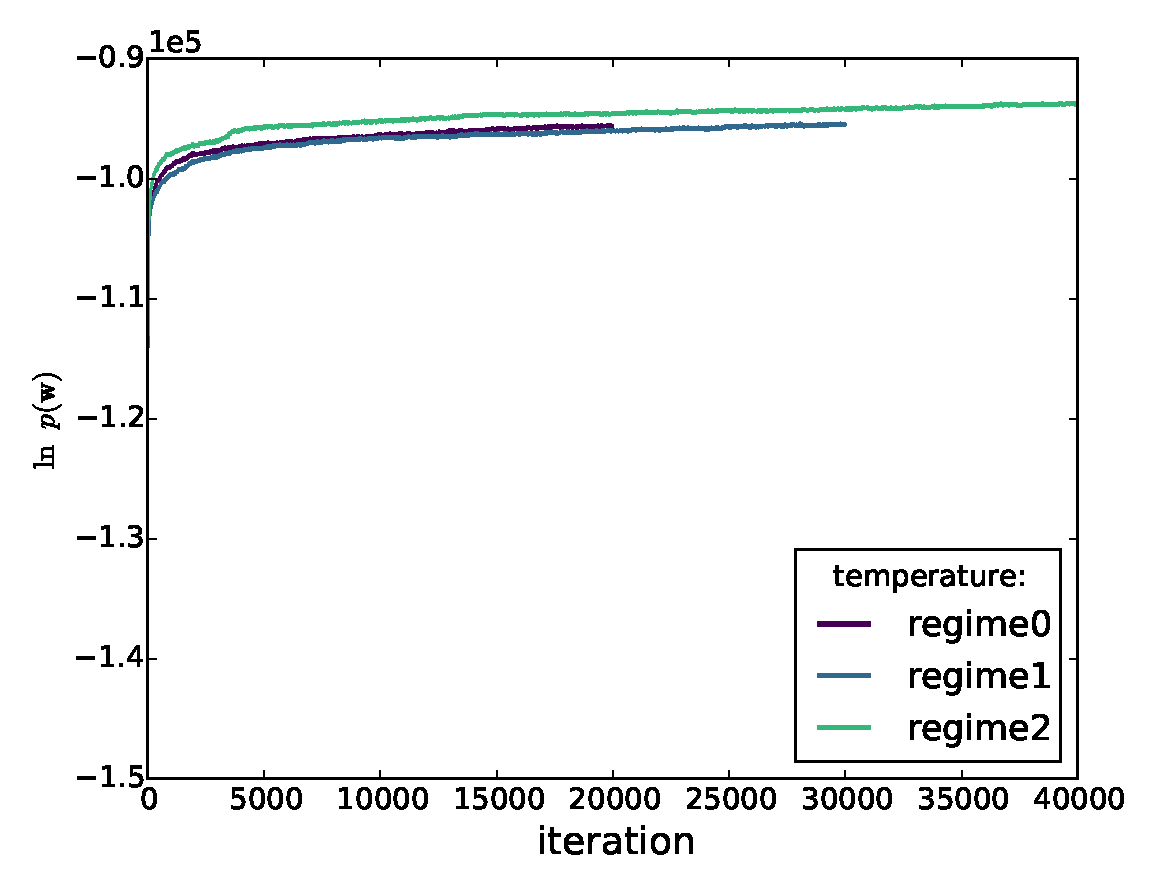
\includegraphics[width=0.5\textwidth]{images/temperature-log_prob}
    \captionof{figure}{The effect of temperature regime on the log joint probability over time.}
	\label{fig:temp_logprob}
\endgroup

\subsubsection{Initialization strategy}

Figure \ref{fig:init_logprob} shows the effect of initialization strategy on the log joint probability over time. It shows that initializing the model the maximum number of boundaries results in the highest final joint probability. Note that initializing the model with the true boundaries results in a lower joint probability, although initially it gets the highest joint probability, unsurprisingly.

\begingroup
    \centering
    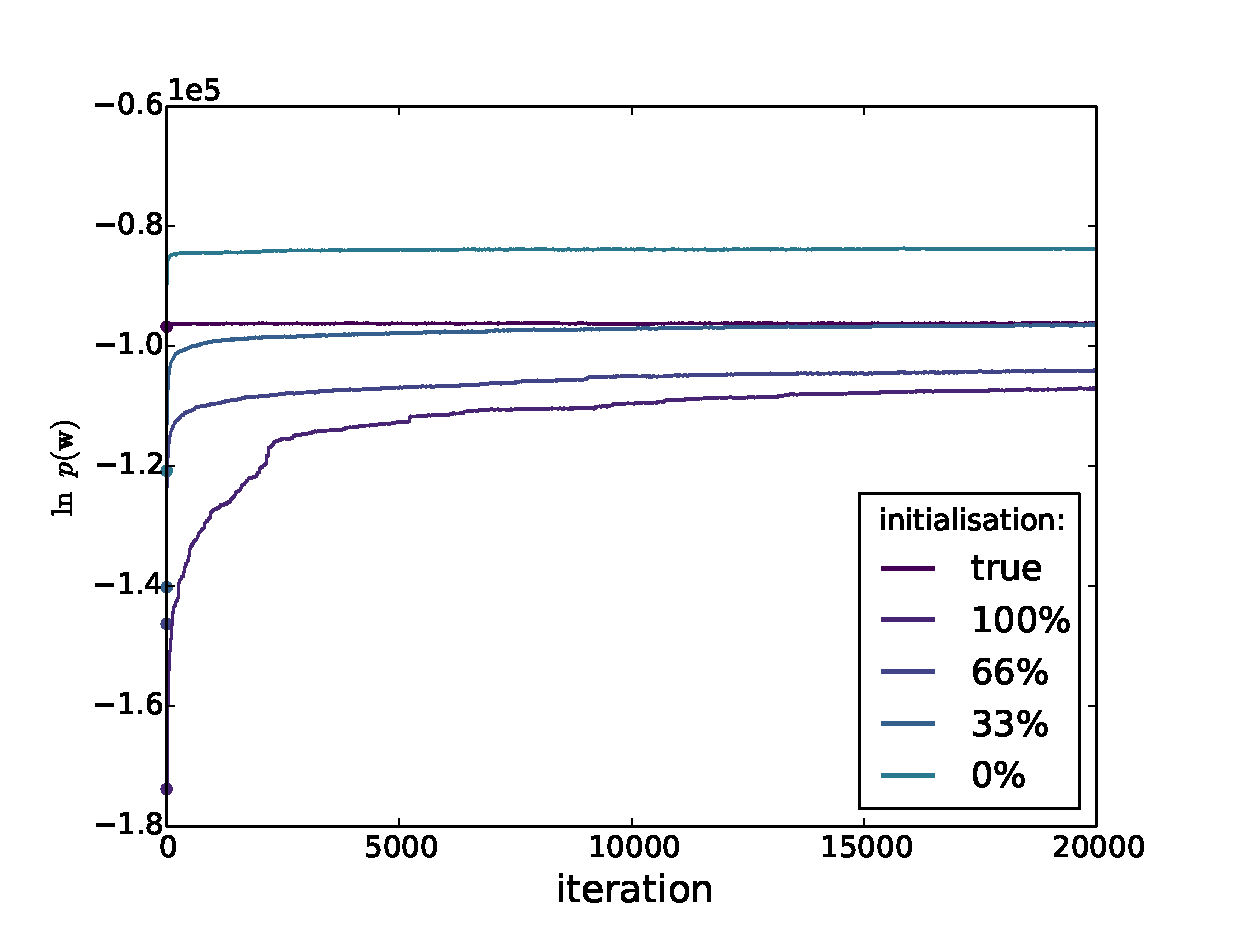
\includegraphics[width=0.5\textwidth]{images/initialisation-log_prob}
    \captionof{figure}{The effect of initialization strategy on the log joint probability over time.}
    \label{fig:init_logprob}
\endgroup

\subsection{Model parameters}

Figure \ref{fig:model_parameters} shows the effect of different model parameter choices on the $F_0$-measure, evaluated on words, boundaries and the lexicon. The effect is mostly visible at the lexicon level, favoring higher values for both $\alpha_0$ and $p_\#$, but it does not seem to affect the $F_0$-measure of the words and boundaries much.

%\end{multicols}{2}
\begin{figure}[!ht]
\begin{tabular}{cccc}
\subfloat[$F_0$ for different values of $\alpha_0$]{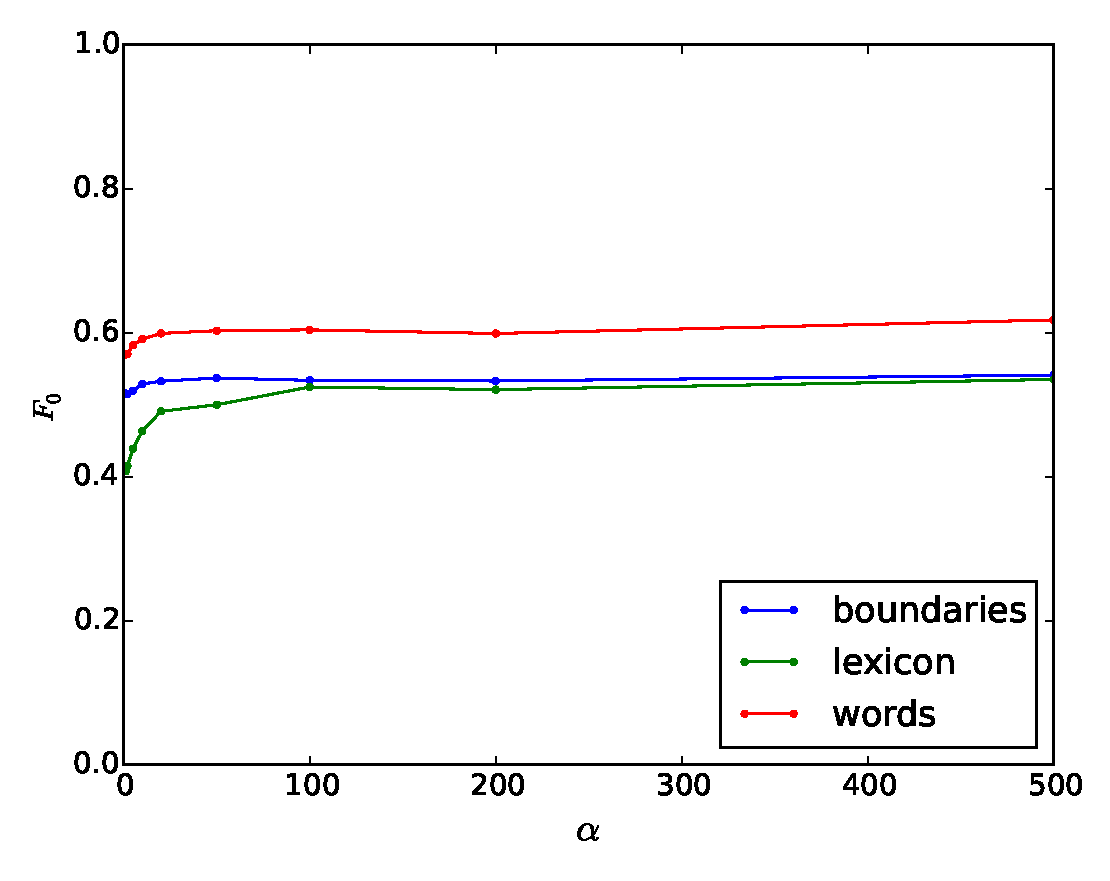
\includegraphics[width=0.47\linewidth]{images/alpha-f0}} &
\subfloat[$F_0$ for different values of $p_\#$]{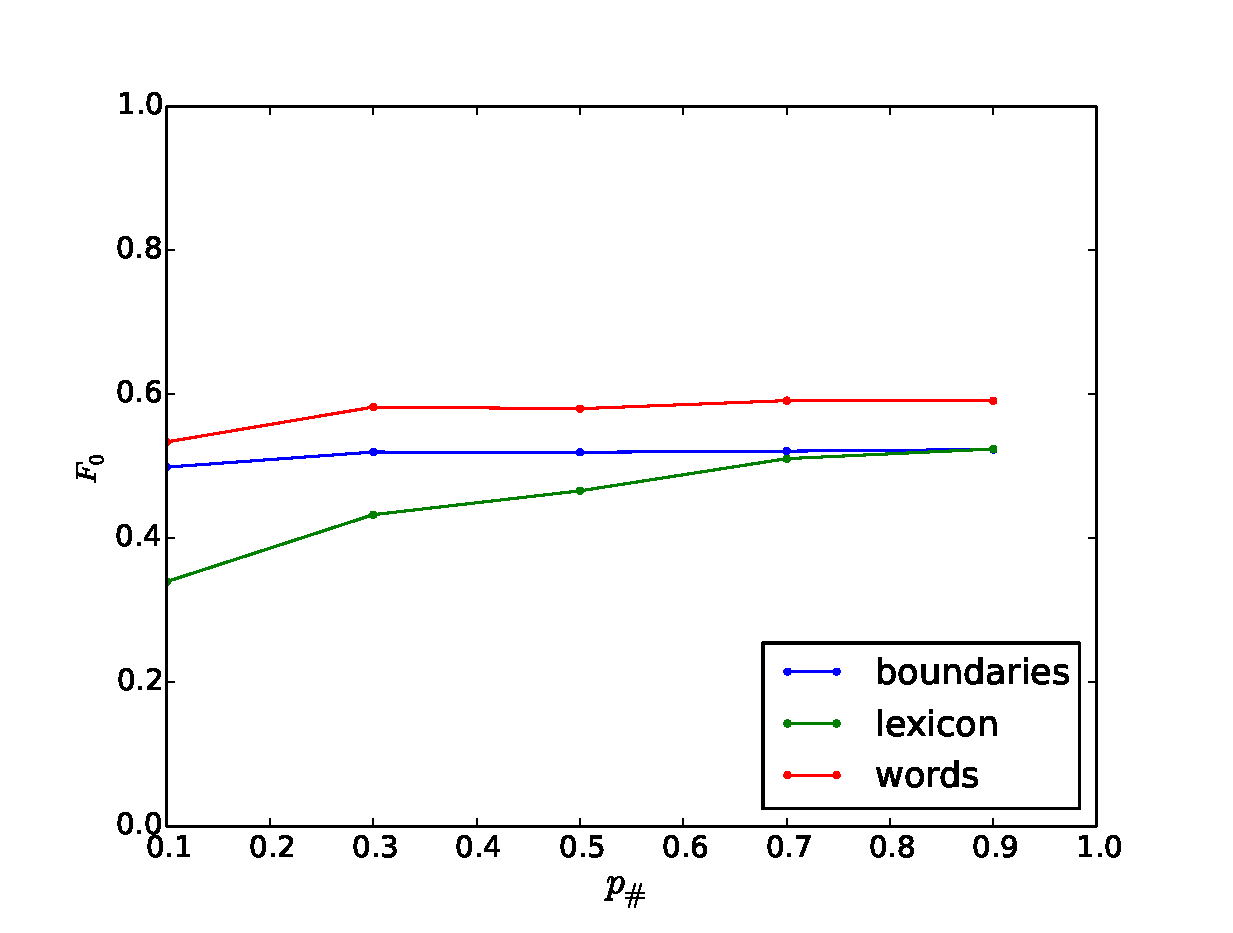
\includegraphics[width=0.47\linewidth]{images/p_dash-f0}}
\end{tabular}
\caption{The effect of different values for $\alpha_0$ and $p_\#$ on retrieval quality evaluated on words, boundaries and the lexicon.}
\label{fig:model_parameters}
\end{figure}
%\begin{multicols}{2}

Table \ref{tab:model_params} shows the retrieval quality of the model evaluated on words, boundaries and lexicon.

\begin{table}[]
\centering
\caption{Retrieval quality of the model with $\alpha_0 = 20$ and $p_\# = 0.5$ evaluated on words, boundaries and lexicon.}
\label{tab:model_params}
\begin{tabular}{llll}
\hline
                    & \textbf{Precision} & \textbf{Recall} & {$\mathbf{F_0}$} \\ \hline
\textbf{Words}      & 0.61               & 0.59            & 0.59          \\
\textbf{Boundaries} & 0.59               & 0.51            & 0.53          \\
\textbf{Lexicon}    & 0.50               & 0.48            & 0.49          \\ \hline
\end{tabular}
\end{table}

%\FloatBarrier

\subsection{Qualitative results}

To find out why the model does not perform perfectly, we must analyze the segmentation that it produces. Below are some good and bad examples.\\


\begin{multicols}{2}
\noindent\textbf{Good examples}

\begin{itemize}
\item \texttt{fid It} (actual)\\ \texttt{fid It} (retrieved)
\item \texttt{pUt It In oke} (actual)\\ \texttt{pUt It In oke} (retrieved)
\item \texttt{oke} (actual)\\ \texttt{oke} (retrieved)
\item \texttt{gIv hIm 6 kIs oke kAm an} (actual)\\ \texttt{gIv hIm 6 kIs oke kAm an} (retrieved)
\item \texttt{lUk} (actual)\\ \texttt{lUk} (retrieved)
\item \texttt{D\&t} (actual)\\ \texttt{D\&t} (retrieved)
\item \texttt{WAt 6 n9s dOgi} (actual)\\ \texttt{WAt 6 n9s dOgi} (retrieved)
\item \texttt{lEts si nQ hu goz W* D\&ts WAt 9d l9k tu no} (actual)\\ \texttt{lEtssi nQ hu goz W* D\&ts WAt 9d l9k tu no} (retrieved)
\end{itemize}
\vfill
\columnbreak
\noindent\textbf{Bad examples}

\begin{itemize}
\item \texttt{D\&ts r9t} (actual)\\ \texttt{D\&tsr9t} (retrieved)
\item \texttt{Ol r9t nQ WAt wUd yu l9k} (actual)\\ \texttt{Olr9t nQWAt wUdyul9k} (retrieved)
\item \texttt{WAt dId yu du t6de} (actual)\\ \texttt{W AtdIdy udut6de} (retrieved)
\item \texttt{WAt Els wUd yu l9k} (actual)\\ \texttt{WAtEls wUdyul9k} (retrieved)
\item \texttt{WAt Iz D\&t} (actual)\\ \texttt{WAtIzD\&t} (retrieved)
\item \texttt{wUd yu l9k D6 dOgi} (actual)\\ \texttt{wUdyul9k D6dOgi} (retrieved)
\item \texttt{k\&n yu rid 6 bUk} (actual)\\ \texttt{k\&nyu ri d6bUk} (retrieved)
\item \texttt{v*i gUd} (actual)\\ \texttt{v*igUd} (retrieved)
\end{itemize}

\end{multicols}

We see that the good examples consist mostly of very short utterances, which are arguably easier to segment than longer utterances. The bad examples consist mostly of quite long utterances, and we can clearly see that they all lack some boundaries. The boundaries that the model did find in these cases, are mostly correct. In other words, the model under-segments these utterances.

\subsection{PYP Model}

\subsubsection{Comparison to DP model}
Figure \ref{fig:PYPvsDP} shows the comparison between the DP model and the PYP model with the $\beta$ parameter set to zero. It can be seen that the models perform equally well. A investigation of the corpus probability over time showed that the convergence of both models was also similar.

\begingroup
    \centering
    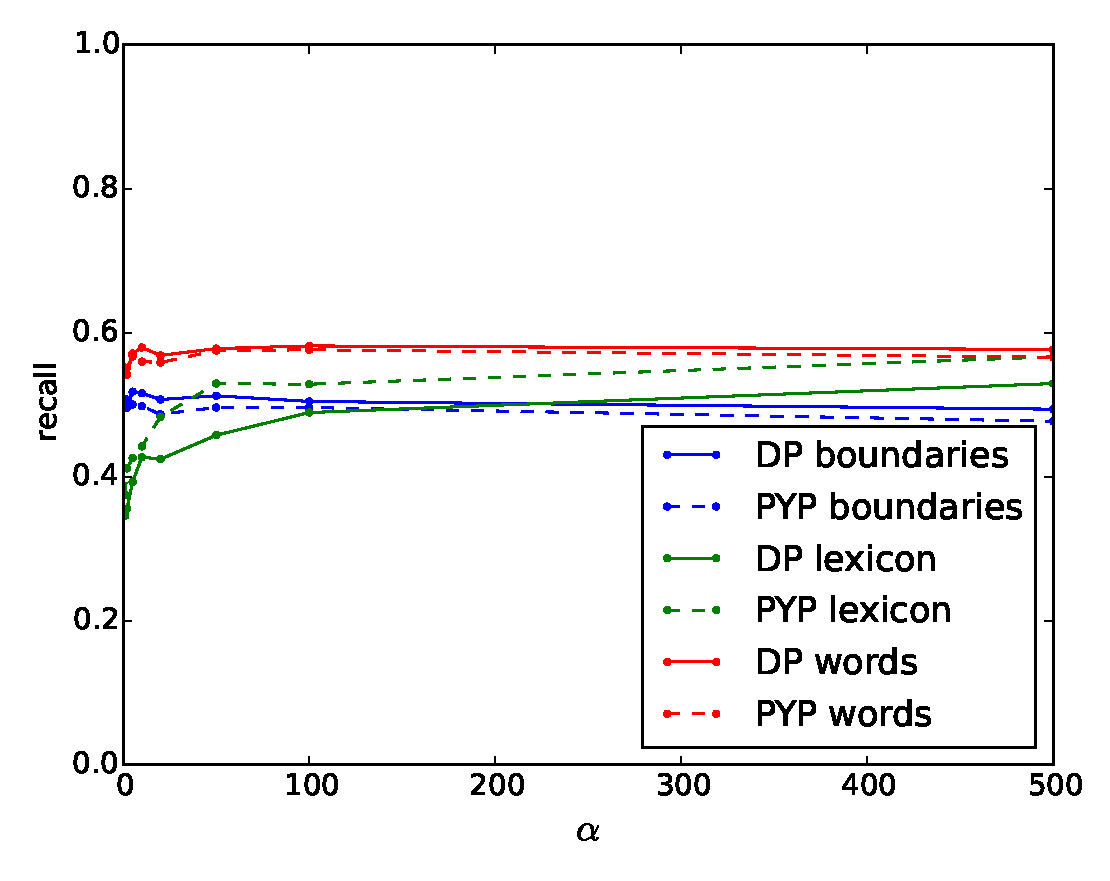
\includegraphics[width=0.5\textwidth]{images/DP-vs-PYP-recall}
    \captionof{figure}{A comparison of the DP model with the PYP model (with $\beta$ set to 0)}
    \label{fig:PYPvsDP}
\endgroup

\subsubsection{Parameter settings}
Figure \ref{fig:gridF0} shows the results of a grid search for different values of $\alpha$ and $\beta$. It can be seen that for each of the three measures, the best results are achieved when $\beta$ = 0. When $\beta$ is set to another value, performance decreases dramatically.
Figure  shows the comparison between the DP model and the PYP model with the $\beta$ parameter set to zero. It can be seen that the models perform equally well. A investigation of the corpus probability over time showed that the convergence of both models was also similar.

\begingroup
    \centering
    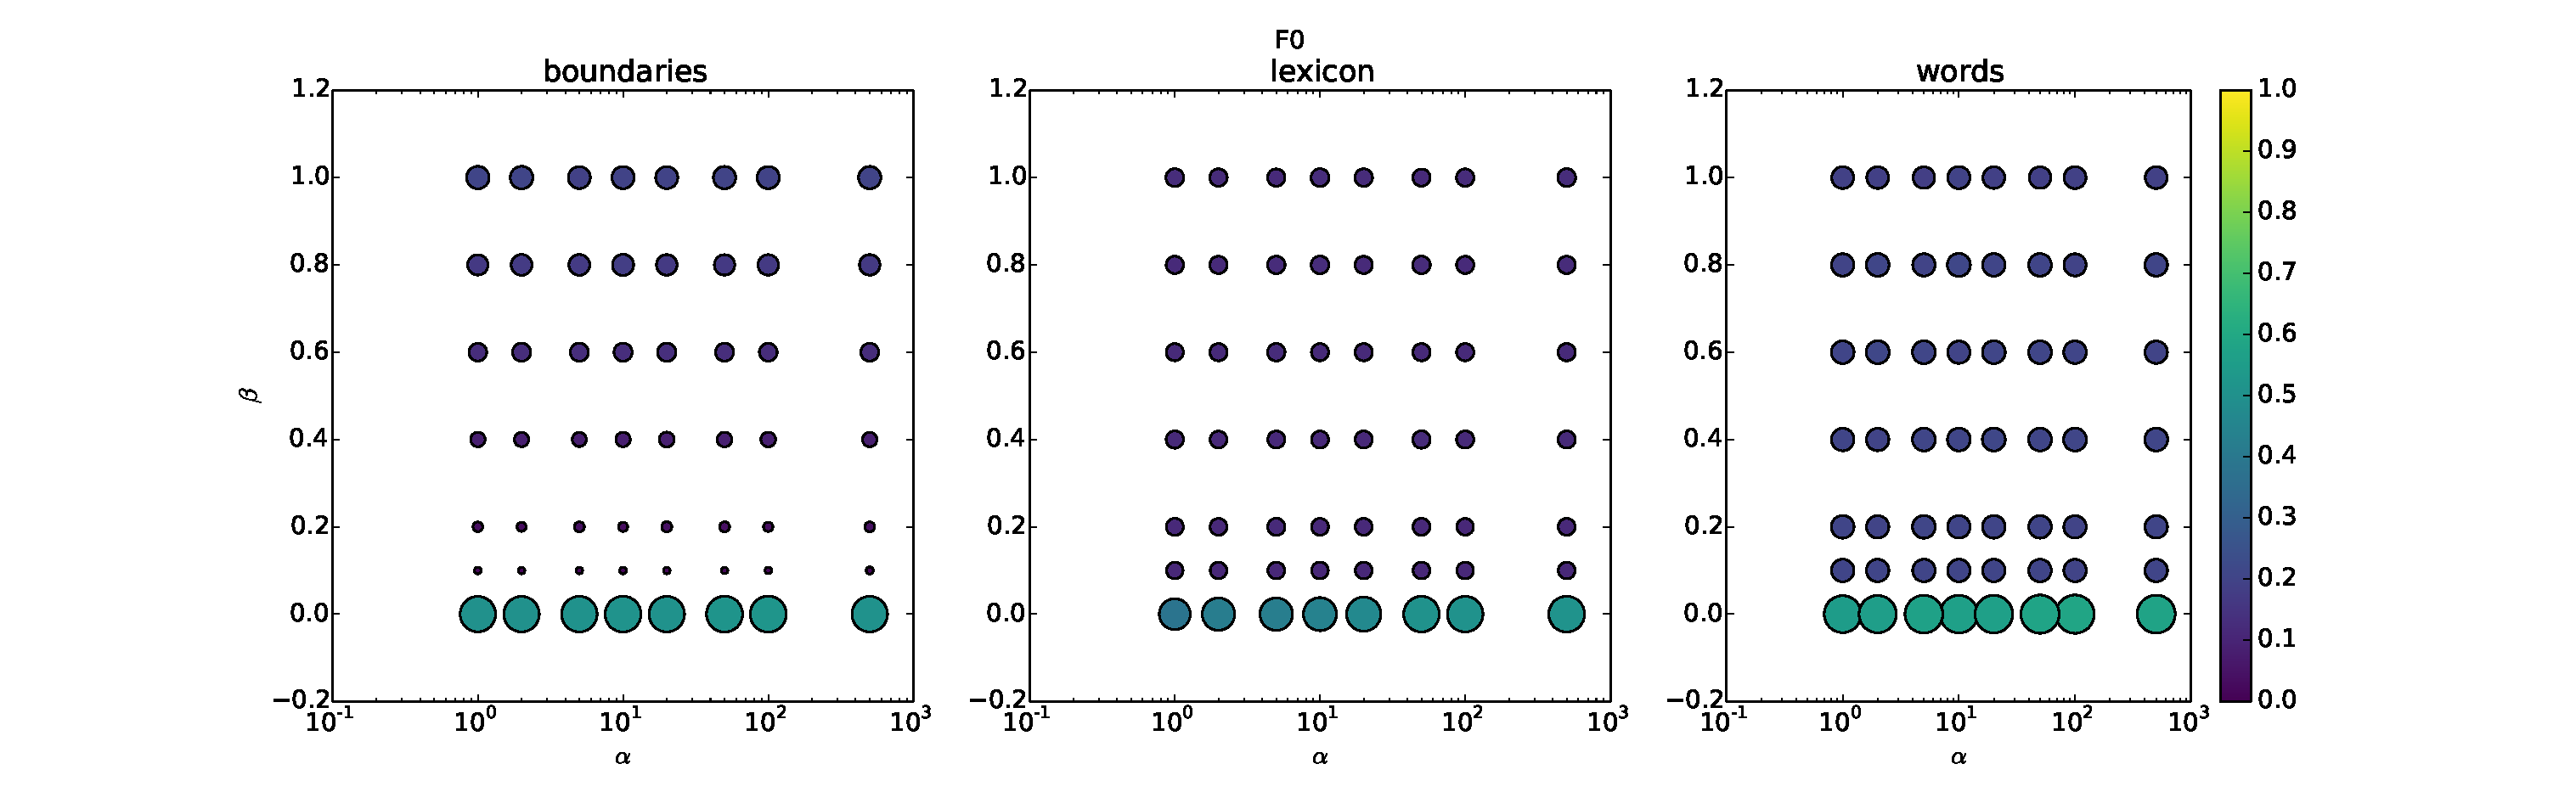
\includegraphics[width=0.9\textwidth]{images/PYP-F0}
    \captionof{figure}{$F_0$ scores for different values for $\alpha$ and $\beta$ using the PYP model.}
    \label{fig:gridF0}
\endgroup

\subsubsection{Seating arrangement}
Figure \ref{fig:PYPiter} shows the evolution of the seating arrangement over time.
The most salient result is that the patterns for each measure are very different for $\beta=0$ and all other values of $\beta$.

For all measures, we see a convergence for $\beta = 0$, to a value that is very different from the original value. For any other value of $\beta$, there is a small change in the first iteration, but from then on, all measures remain constant across iterations.

The number of types, the number of tokens and the number of tables ($K$) decreases as the iterations progress. All these measures increase for higher values of $\beta$.

In general $\beta=0$ commits to this trend, except for the number of tokens, which is high compared to other values of $\beta$.

\begingroup
    \centering
    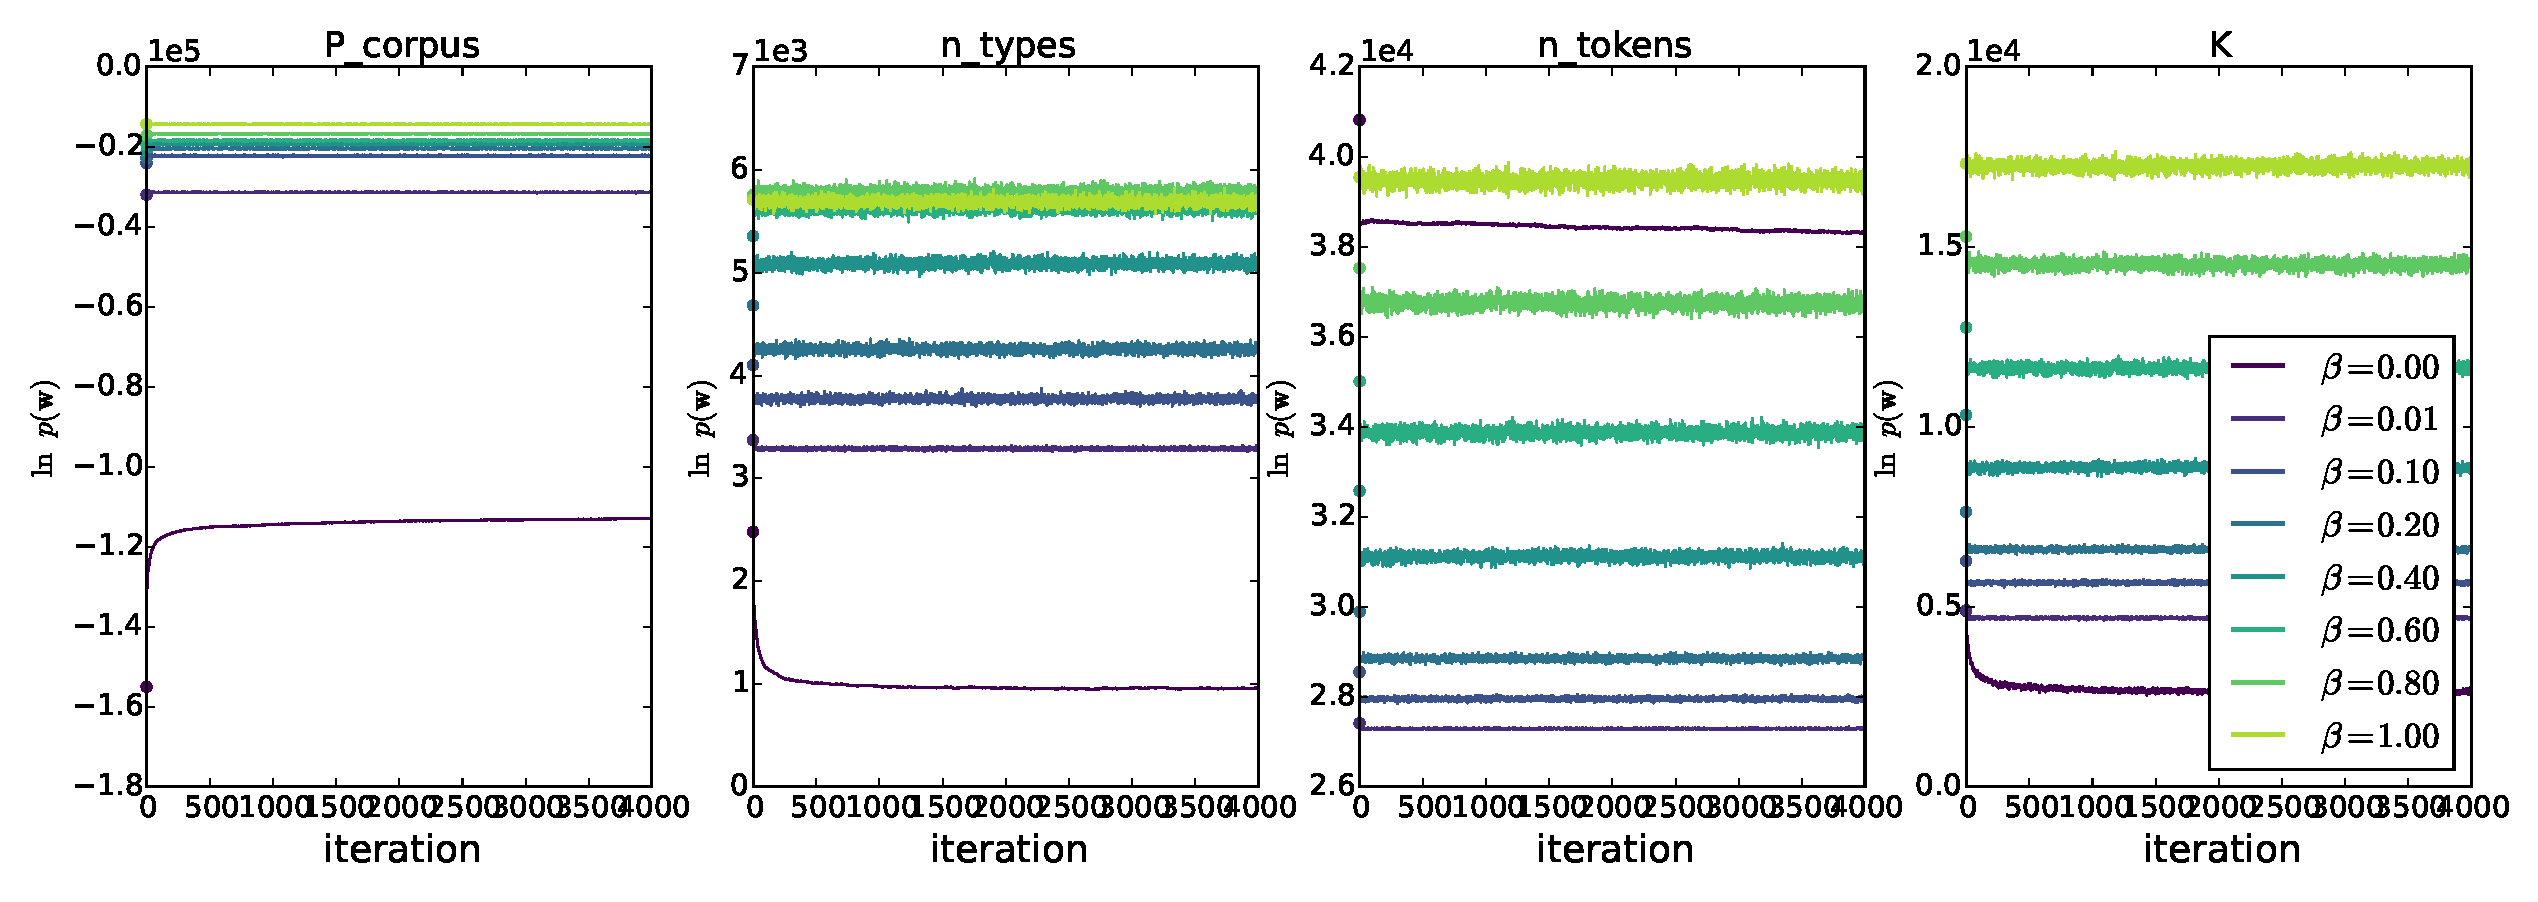
\includegraphics[width=0.9\textwidth]{images/PYP-iter_plots}
    \captionof{figure}{The evolution of various seating arrangement measures over time, for different values of $\beta$, $\alpha$=2 for all graphs.}
    \label{fig:PYPiter}
\endgroup


\section{Conclusion}

In this project, we reproduced the unigram model of \cite{Goldwater200921} and attempted to replicate their results. While we were unable to exactly match their results, our results generally seem to agree with their results. Moreover, our results show that our model suffers from the same problem as their unigram model, namely that it tends to under-segment the corpus. This confirms their main finding that the word-to-word independence assumption is inadequate and should be dropped or changed.
Extending the DP unigram model to a PYP model did decrease the performance. Further research should investigate what causes this effect.

\section{Discussion}

Of all the experiments, the initialisation strategy shows the largest effect on performance. Although initialising the corpus with the true segmentation results in the highest probability before sampling, a higher probability is reached using other initialisations. The fact that there are higher probabilities than the true segmentation does indicate a fundamental limitation of our model.

A worrying finding is the fact that initialisation has a large effect on the corpus probability after running the sampler. This indicates that our sampler does not converge to a global optimum but get's stuck locally. Furthermore, this finding is not in line with \cite{Goldwater200921} who found no effect of initialisation. 

Moreover, we note that although the initialization with true boundaries has the highest joint probability on the corpus initially, it does not get the highest final joint probability. Assuming the true segmentation of the corpus is correct, we conclude that the model is in fact inadequate for this problem. This suggests that the assumption that words are independent units may not be a realistic assumption, and should be dropped or changed (to e.g. the bigram assumption). 

Interestingly, the probability of the true initialisation does not change after sampling, but remains constant indicating that the true segmentation is in fact a local optimum. Furthermore, fewer boundaries result in a higher probability with the best probability found when no boundaries are initialised. This initialisation corresponds to the trival MLE segmentation where each utterance is seen as a token.

Varying the parameters only has marginal effects. The temperature regime can slightly improve learning speed and performance, but it does not make a big difference. The $\alpha_0$ parameter should not be too small, but after a certain value (e.g. $\alpha_0 > 20$), it does not really affect retrieval quality anymore. The same applies to the $p_\#$ parameter, where values greater than 0.5 are preferable. Finally, the fact that the lines in most graphs don't seem to converge, suggests that the model may be stuck in a local optimum.

The numeric results of our experiments do not directly match those of \cite{Goldwater200921}, but they are similar. We suspect that these differences may be caused by small implementation differences. However, our model suffers from the same problem as their unigram model: it tends to under-segment the corpus. Thus, our results confirm an important finding of \cite{Goldwater200921}, which is that the assumption that words are independent of each other is most likely inadequate.

Taken altogether, the DP unigram model does not perform very well on this task, in line with the findings of  \cite{Goldwater200921}. We suggested the PYP as an improvement to this model, but in fact, the PYP model worsened performance. Either the model and parameters were not implemented correctly, or the PYP model is actually not suited for this task. We conducted several experiments to investigate both options.

With $\beta$ set to 0, the model behaves as the DP model, as expected. This indicates that the of modelling $h^-$ is implemented correctly. Another expected finding is that higher $\beta$ values result in an increased number of clusters ($K$). 

However we also found some unexpected effects of the $\beta$ parameter. First of al, lower the values of $\beta$ results in decreased performance. As the highest performance was found for $\beta = 0$, this finding is counter intuitive, and may indicate an implementation error.

As expected, larger $\beta$ values result in more clusters. The number of types also increases with $\beta$, which means that not only do we have more clusters per type, but there also are more different labels. Surprisingly the number of tokens increases with $\beta$ as well. Taken together with the qualitative results, we conclude that the model does still under-segment but also makes many incorrect segmentations.

The different values of $\beta$ also have a large effect on corpus probability, even after initialisation. This may mean indicate an implementation error and may be due to the fact that we defined the corpus probability as $p(\vt{w}|\vt{z})$ instead of including the distribution over $\vt{z}$. However the same probability is used in \cite{Goldwater200921} for the bigram model. Analogous to our PYP model, the seating is modelled explicitly for the bigram model. The probability of \cite{Goldwater200921} does converge nicely, which means that our equations for $p(w_i | \wmin, \vt{z}^-)$ may be incorrect.
 
 Besides possible implementation errors, our finding may imply that the PYP model is not suited for this task. It could be the case that the distribution of types and tokens in infant directed language is not distributed according to the power-law. In fact, this may very well be the case, as the vocabulary of our corpus is rather limited. 
 Furthermore, our findings may indicate that the assumption of the distribution over words that is implied by the PYP is not an assumption that an ideal learner should make in order to find the right clustering. However, more sanity checks and control experiments have to be conducted to find out what exactly is causing our results.

Bla bla \cite{Goldwater200921} %Just a placeholder to make it appear in the bibliography
%\nocite{*}
\bibliographystyle{plain}
\bibliography{report.bib}

\end{document}
